\chapter{关系数据库模式与本体间映射的问题描述}
\label{chap01}

\section{相关工作}

现有工作从多个方面研究了关系数据库模式和本体间的映射问题,例如设计映射系统的框架
、提出具体映射算法以及定义映射结果的语法语义。有关介绍请参见研究综述\cite{4,7}。
根据是否给定本体,现有工作可分为如下两类:

\begin{itemize}
	\item 从已有关系数据库模式中采用信息抽取的方法生成新的本体
	\item 发现已有关系数据库和给定本体之间的关联
\end{itemize}

第一类工作主要针对本体不存在的情况,如Relational.OWL\cite{33}可将关系数据库自动翻
译为OWL Full本体,将关系数据库模式中的关系和属性分别表示为元类Table和Column的实例
,将关系数据库中元组表示为代表模式的类的实例。类似工作DataMaster\cite{34}和ROSEX
\cite{35}在Relational.OWL的基础上进行了扩充。D2RQ\cite{11}利用了逆向工程的方法和
一些预先定义的规则,可将关系数据库模式自动化地翻译为RDFS本体,并且允许用户参与修
正映射结果。文献\cite{13}定义了一组Datalog的规则,可将关系数据库模式及其实例数据
直接映射为新的本体,并且证明这种直接映射具有信息保持、查询保持以及单调性的性质,
而后又针对语义保持的性质提出两种改进直接映射,最终得到单调性和语义保持不能共存的
结论。

第二类工作针对给定本体的情况,如DartGrid是一个中医药领域的数据集成系统\cite{25},
其中的DartMapping模块提供了一个可视化的工具,帮助领域专家手工定义关系数据库模式与
本体间的映射。OntoMat-Reverse\cite{26}使用逆向工程规则和基于编辑距离的文本相似度
计算方法,半自动地发现关系数据库中表/列和本体中类/属性间的映射,与它类似的工作还
有RONTO\cite{27}、Marson\cite{24}等。OntoGrate框架\cite{28}首先将每个关系数据库模
式转化为对应的DB本体,然后借助记录链接和多关系数据挖掘等技术,高度自动化地发现DB
本体和其他语义网本体之间的映射。此外OntoGrate还设计了一种称为Web-PDDL的映射语言,
将针对本体的查询转换为SQL查询。类似地,StdTrip\cite{29}也是将关系数据库模式转化
为本体后再实施本体映射。MapOnto\cite{10}使用树状结构作为数据库模式和本体的中间转
换模型,基于预先发现的简单映射,在两个中间模型上迭代地传播这些映射,最终发现关系
数据库模式中元素和本体元素之间的多对多映射,并以Horn字句的形式表达。Marson则基于
具有分类特性的关系数据库列(例如性别的取值有``男''和``女''),运用决策数算法构造
一类具有包含关系的复杂映射,可以转化为基于视图的查询。

对比上述研究工作,在简单映射发现方面,本文提出了基于虚拟文档的方法,通过考察元素周
围的各种邻居元素的自然语言描述,显著提高了映射结果的效果。在复杂映射学习方面,除
MapOnto和Marson以外,其它工作还很少考虑复杂映射。MapOnto仅利用属性的定义域/值域
的兼容性构建一种句法层次上的复杂映射,Marson则是基于具有分类特性的列构造一类包含
查询,而本文运用归纳逻辑编程算法,能够从重叠实例数据中学习出多种复杂映射,覆盖面更
广。另外,数据库领域中的模式映射\cite{30}和语义网领域中的本体映射\cite{31}已经有
不少有借鉴意义的相关研究,也有工作试图将数据库模式转换为本体后再寻找映射
\cite{28,29},但是由于关系数据库模式和本体之间不存在完美的兼容关系,所以这种转换
通常是不完备的,造成了后续本体映射的精度损失。


\section{问题描述}

数据模型是在概念层面对数据进行的描述和定义,隐藏了许多低层次的存储细节\cite{9}。
对某一类数据的结构、联系和约束的描述称为数据模式。关系数据库和本体基于两种不同的
数据模型,本文主要研究这两种异构数据模型之间的映射发现。

关系数据库模式是一个关系模式的有限集合。一个关系模式由关系名、关系中的属性名及其
关联的定义域组成。关系模式中的定义域包含定义域名和一个取值的集合。关系数据库模式
中的完整性约束定义了施加在数据上的语义约束。本文用$R$表示一个关系(relation),
$A$表示一个属性 (attribute)。$type(A)$表示$A$的定义域名,$rel(A)$表示$A$所属的
关系。$pk(R)$表示R中的主键,$ref(A)$表示$A$引用的属性。


本体是对某一概念模型的显式规范说明。如果没有特别说明,文章所涉及的本体是指使用
OWL语言\cite{6}描述的语义网本体。使用$C$表示一个本体类(class),$P$表示一个属性
(property)。$P_d$表示一个数据类型属性(data type property),$P_o$表示一个对象
属性(object property)。$d(P)$表示$P$的定义域,$r(P)$表示其值域。

在信息数据集成、数据仓库中的数据集成等研究中,Horn子句常被用于表达关系数据
源和以描述逻辑表示的概念模型之间的联系\cite{10}。一个Horn子句是一组文字
(literal)的析取,其中文字是应用到常量或变量上的谓词。能够被满足的(与事实相符
的)文字被称作正文字,否则是负文字。一个子句被称为Horn子句当且仅当它最多有一个正
文字。Horn规则是一种Horn子句,仅包含一个正文字和至少一个负文字,可以表示成
$H \mbox{:-} L_1 \wedge L_2 \wedge \ldots \wedge L_k $的形式,其中$H$称为规则头
或者后继,$L_1 \wedge L_2 \wedge \ldots \wedge L_k$称为规则体或者前驱。本文基于
Horn规则来定义关系数据库模式与本体间的语义映射。

\newtheorem{defn}{\heiti{定义}}
\begin{defn}[关系数据库模式与本体间映射]
一个关系数据库模式$\mathcal{S}$和一个本体$\mathcal{O}$之间的映射发现一个语义映射
集合$\mathcal{M}=\{m_1,\ldots,m_n\}$。每个$m_i(1 \le i\le n)$表示成一个Horn规则
的形式:$T(\overrightarrow{X}) \mbox{\rm:-} \varPhi (\overrightarrow{X},
\overrightarrow{Y}) $,其中$T(\overrightarrow{X})$
表示$\mathcal{S}$中的一个关系R的单个|R|元谓词文字,|R|为R中属性的数量;而
$\varPhi (\overrightarrow{X},\overrightarrow{Y})$是由$\mathcal{O}$中表示类的一
元谓词文字和表示属性的二元谓词文字构成的合取式。
\end{defn}

请注意,本文研究假设目标本体和关系数据库模式均已独立存在,而以D2RQ\cite{11}和
文献\cite{12,13}为代表的工作则是针对本体不存在的情况,考虑如何将关系数据库模式
转换为新本体,与本文工作有本质区别。

\section{关系数据库模式和本体实例}
为方便理解,以下给出一个关系数据库模式和一个本体的例子。

图\ref{fig:onto}为一个本体,包含了4个类:
\emph{Course}、\emph{Student}、\emph{Undergraduate}和\emph{Graduate}, 其中
\emph{Undergraduate}和\emph{Graduate}是\emph{Student}的子类;6个属性:
\emph{takesCourse}、\emph{taOf}、\emph{hasSID}、\emph{hasStudentName}、
\emph{hasCID}和\emph{hasCourseName},其中前两个属性为对象属性,其余为数据类型
属性。


\begin{figure}[htbp]
\centerline{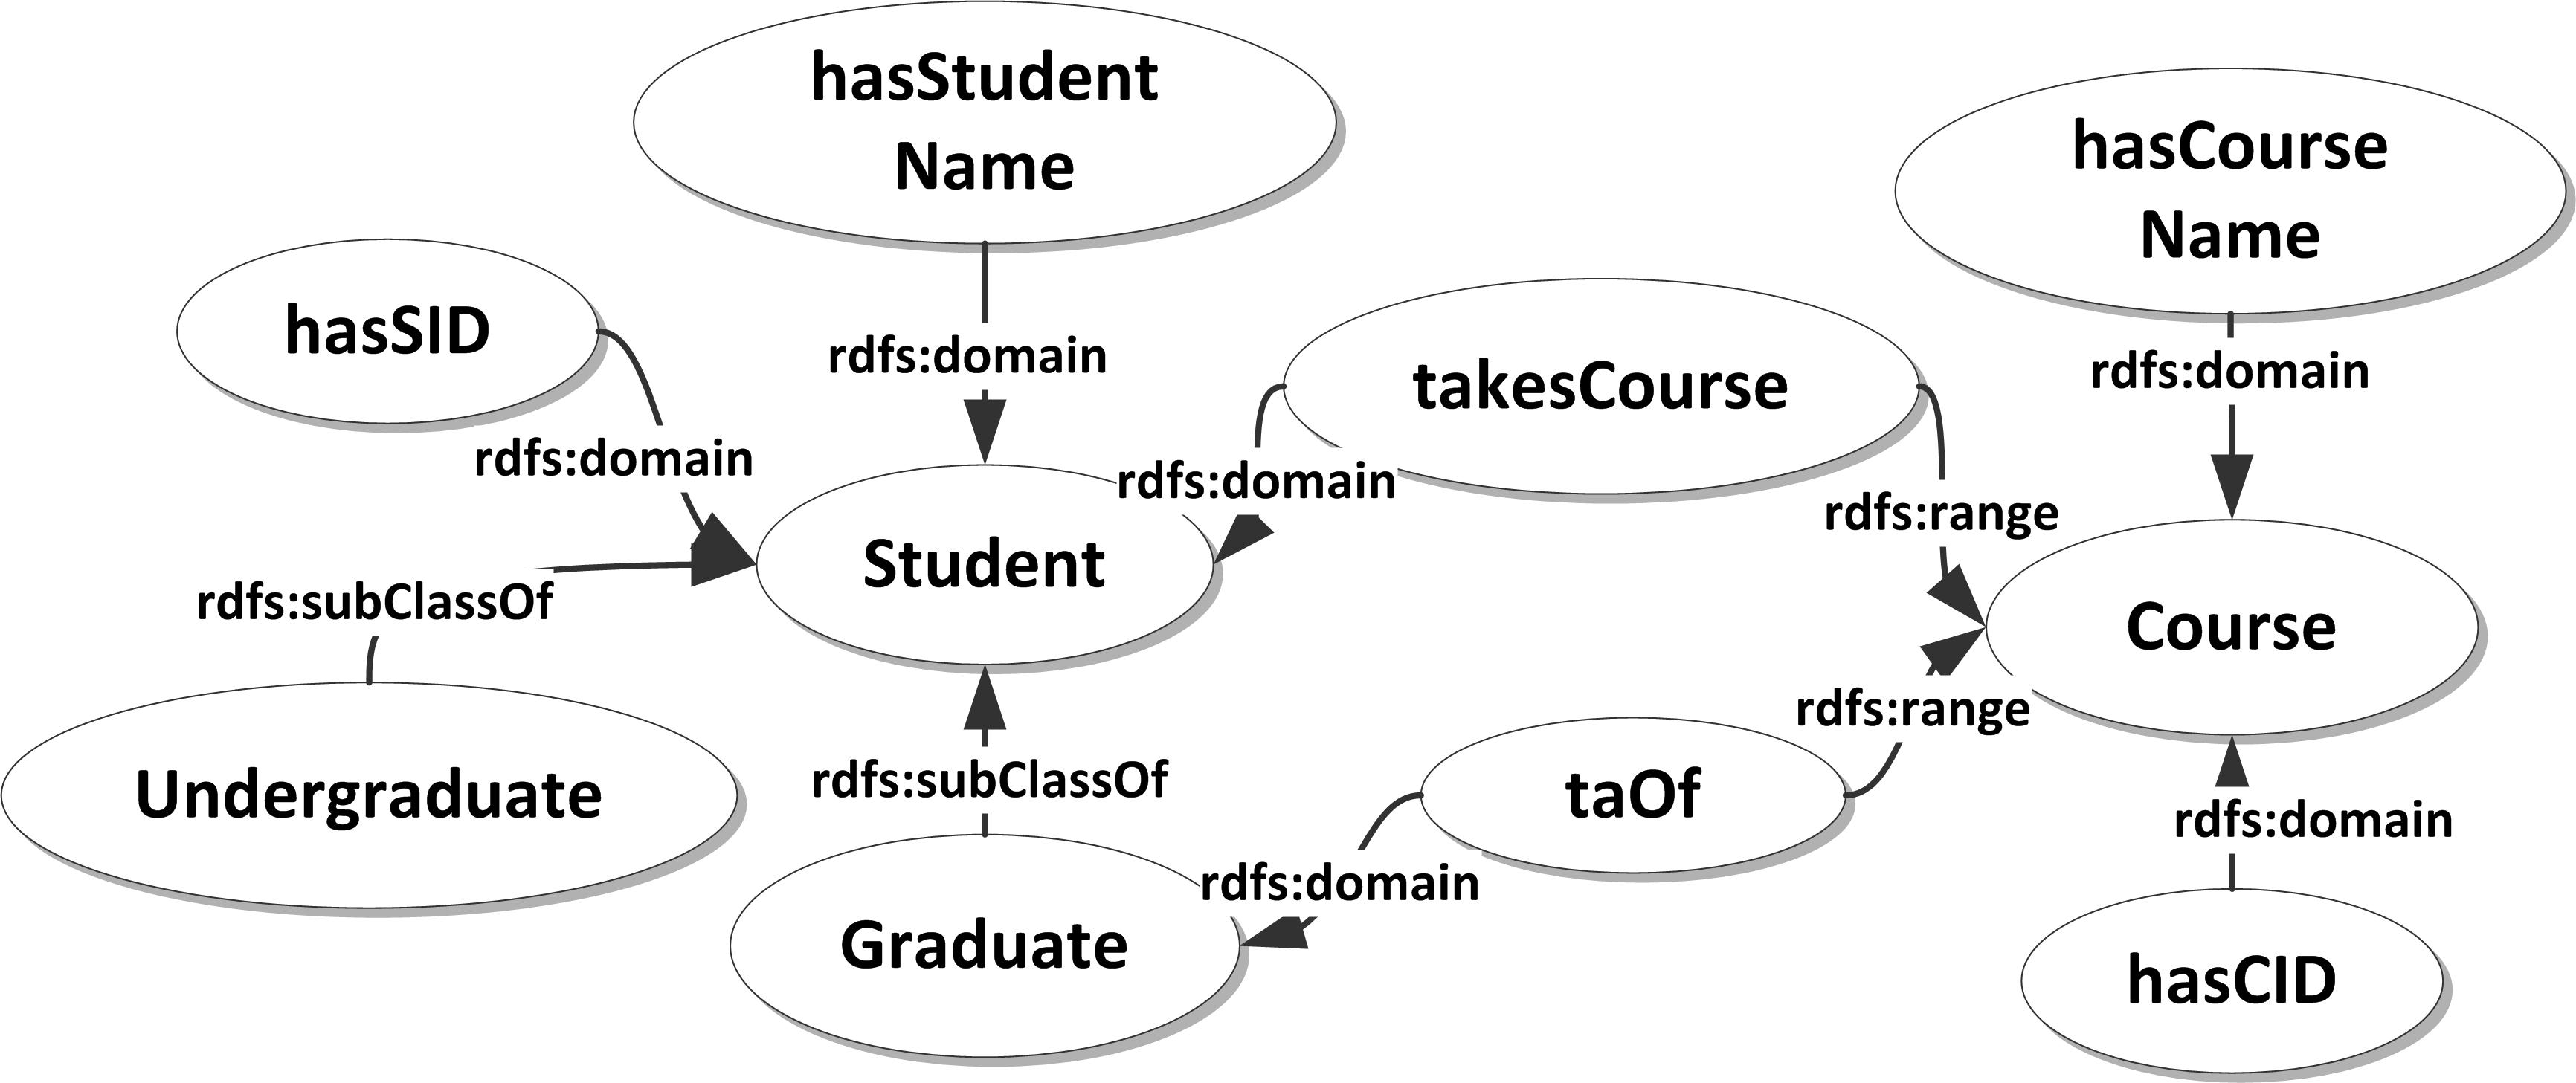
\includegraphics{ontology}}
\caption{本体示例}
\label{fig:onto}
\end{figure}

图\ref{fig:db}为一个关系数据库模式,包含3个关系:\emph{student}、\emph{course}
和\emph{takes\_course};带下划线的属性为关系的主键,比如\emph{student}中的
\emph{\underline{sid}};箭头表示引用完整性约束,例如\emph{takes\_course}中外
键\emph{\underline{cid}}引用了\emph{course}中的\emph{\underline{cid}}。

\begin{figure}[htbp]
\centerline{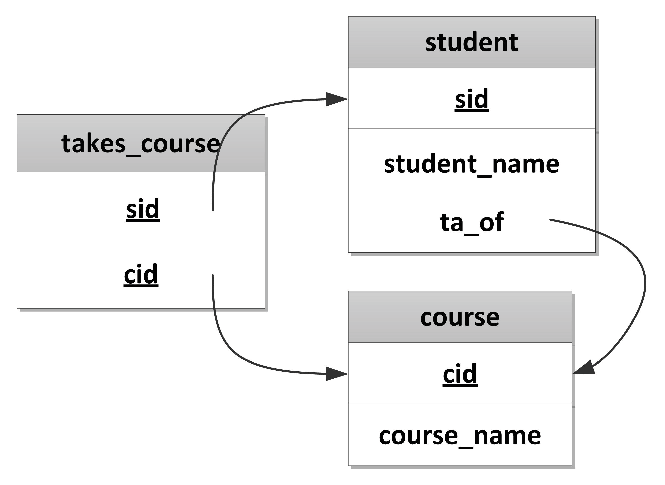
\includegraphics[height=5cm]{DB}}
\caption{关系数据库模式示例}
\label{fig:db}
\end{figure}


构建图\ref{fig:db}中关系数据库模式和图\ref{fig:onto}中本体间的映射,既可以发
现简单映射,如
$\mathcal{S}$:\emph{Course.course\_name}和$\mathcal{O}$:\emph{hasCourseName};
也可以发现复杂映射,如$\mathcal{S}$:\emph{student}(\emph{sid,\_,\_}) 
:- $\mathcal{O}$:\emph{Student}(\emph{A}),
 $\mathcal{O}$:\emph{hasSID}(\emph{A,sid})。


